%
% Code Listing
%
\begin{lstlisting} [caption={Useless code},label=useless]
for(int i=0; i<8;i++) 
{
      //donothing
}
\end{lstlisting}


%
% Citation
%
\cite{Sch96:crypt}


%
% Table
%
\begin{table}[h!]
  \begin{center}
    \begin{tabular}{| l c r |}
    \hline
    1 & 2 & 3 \\
    4 & 5 & 6 \\
    7 & 8 & 9 \\
    \hline
    \end{tabular}
  \end{center}
  \caption{A simple table}
\end{table}

%
% Image
%
\begin{figure}[h!]
  \centering
    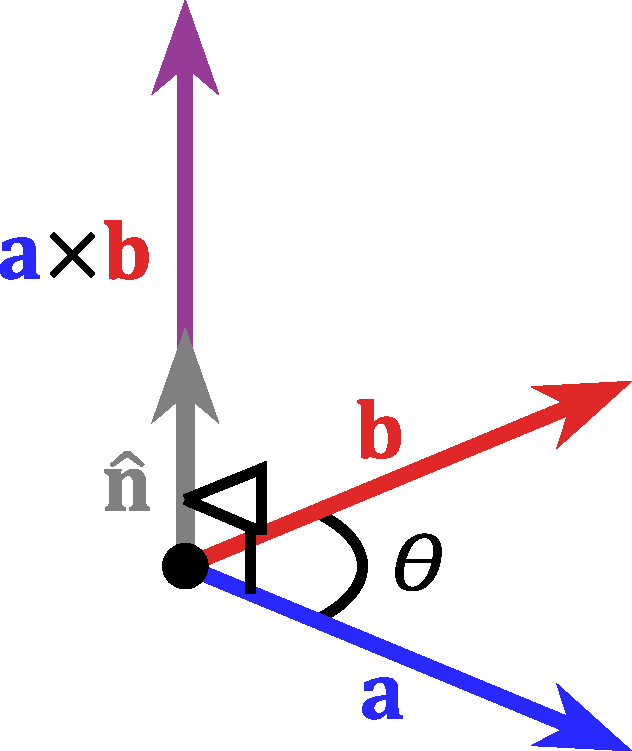
\includegraphics[width=0.3\textwidth]{./img/crossproduct.pdf}
  \caption{Kreuzprodukt zweier Vektoren}
  \label{kreuzprodukt}
\end{figure}

%
% Glossary
% aca: acronym, sample: worterkl�rung
%
A \gls{sample} entry and \gls{aca}. Second use: \gls{aca}.

Plurals: \glspl{sample}. Reset acronym\glsreset{aca}.
First use: \glspl{aca}. Second use: \glspl{aca}.
